
\documentclass[letterpaper, 10 pt, conference]{ieeeconf}  % Comment this line out
\usepackage{graphicx}
                                                          % if you need a4paper

\overrideIEEEmargins
% See the \addtolength command later in the file to balance the column lengths
% on the last page of the document

\usepackage[utf8]{inputenc}
\usepackage[T1]{fontenc}

% The following packages can be found on http:\\www.ctan.org
\usepackage{graphics} % for pdf, bitmapped graphics files
\usepackage{amsmath} % assumes amsmath package installed
\usepackage{amssymb}  % assumes amsmath package installed
\usepackage{tikz}
\usetikzlibrary{positioning}

\title{\LARGE \bf
Clasificación de tumores cerebrales en cortes de MRI con una red neuronal convolucional compacta con control de fuga de datos
}

\author{Miguel Muñoz, David Cardenas y Mario Celis}


\usepackage{etoolbox}
\makeatletter
\def\fnum@table{TABLA~\thetable}
\patchcmd{\thebibliography}{\section*{References}}{\section*{Referencias}}{}{}
\patchcmd{\thebibliography}{{References}}{{Referencias}}{}{}
\makeatother
\begin{document}

\maketitle
\thispagestyle{empty}
\pagestyle{empty}

%%%%%%%%%%%%%%%%%%%%%%%%%%%%%%%%%%%%%%%%%%%%%%%%%%%%%%%%%%%%%%%%%%%%%%%%%%%%%%%%
\section{Introducción}
Los tumores del sistema nervioso central son un grupo heterogéneo cuyo tipo determina el pronóstico y el tratamiento~\cite{c1}. La resonancia magnética (MRI) es la modalidad principal para detectarlos, pero su lectura es lenta y varía entre evaluadores. Por eso, un clasificador automático puede servir para priorizar estudios y como segunda opinión. Este trabajo aborda la clasificación de cortes 2D de MRI cerebral en cuatro clases: glioma, meningioma, tumor hipofisario (\textit{pituitary}) y tejido sano.

Las CNN dominan la clasificación de imágenes desde que los kernels 3$\times$3 apilados~\cite{c2}, la normalización por lotes~\cite{c3} y las conexiones residuales~\cite{c4} permitieron entrenar redes profundas de forma estable. Sobre el conjunto de figshare (3\,064 cortes T1, tres tumores)~\cite{c5}, una CNN propia alcanza 96,56\,\% de \textit{accuracy}~\cite{c6}. Sin embargo, Yagis \textit{et al.}~\cite{c7} mostraron que dividir los datos de MRI a nivel de corte, y no de sujeto, puede inflar el \textit{accuracy} de prueba hasta en 55 puntos porcentuales.

Los objetivos son: (i) construir un \textit{pipeline} reproducible con una partición sin duplicados entre conjuntos; (ii) diseñar y entrenar una CNN basada en bloques de convolución y \textit{max pooling}; y (iii) evaluarla con métricas clínicamente relevantes, cuantificar su variabilidad y el efecto de la fuga, e interpretarla con Grad-CAM~\cite{c9}. Se propone una CNN de 0,29\,M parámetros entrenada desde cero, que obtiene 97,1\,$\pm$\,0,6\,\% de \textit{accuracy} en prueba.



\section{Metodología}
\textbf{Enfoque.} El \textit{pipeline} (notebook adjunto) agrupa y particiona las imágenes, las preprocesa, entrena una CNN compacta desde cero, la evalúa y la interpreta con Grad-CAM.

\textbf{Datos.} Se usa el conjunto \textit{Brain Tumor (MRI Scans)} de Kaggle: 7\,023 imágenes (glioma 1\,621, meningioma 1\,645, \textit{pituitary} 1\,757, sano 2\,000). Su tamaño y clases coinciden con la compilación de~\cite{c10}, que une figshare~\cite{c5} y SARTAJ (tumores) con Br35H (clase sana). Las imágenes tienen 387 tamaños distintos (67,5\,\% de 512$\times$512) y son, en la práctica, de un solo canal. Dos imágenes se agrupan si tienen el mismo MD5, o el mismo dHash y una correlación de Pearson $\geq$0,95 entre miniaturas; así, las 7\,023 imágenes forman 5\,835 grupos. La redundancia es muy desigual: el 52,2\,\% de las imágenes sanas son copias, frente a 0,2--7,3\,\% en los tumores.

\textbf{Partición y preprocesamiento.} La división 70/15/15 (5\,016/1\,004/1\,003), estratificada por clase, se hace \textit{por grupo}: ningún grupo ni duplicado exacto queda en dos particiones. Con una partición aleatoria, 220 imágenes de prueba (22\,\%) tendrían un casi-duplicado en entrenamiento. Aun así, 55 imágenes de prueba (5,5\,\%) comparten un dHash idéntico con una de entrenamiento: no son copias (correlación $<$0,95), sino cortes muy similares, probablemente del mismo paciente. Cada imagen se convierte a gris y se rellena con negro hasta hacerla cuadrada, sin deformar la anatomía. Luego se redimensiona a 128$\times$128 y se normaliza con la media y desviación de entrenamiento (0,179/0,194). Solo en entrenamiento se aplica aumentación: volteo horizontal, rotación $\pm$10$^\circ$, traslación 5\,\%, escala 0,9--1,1 y brillo/contraste $\pm$15\,\%.

\textbf{Arquitectura (Fig.~\ref{fig:arq}).} La red tiene cuatro bloques estilo VGG~\cite{c2}, cada uno con [Conv 3$\times$3--BatchNorm~\cite{c3}--ReLU]$\times$2 y \textit{max pooling} 2$\times$2, con 16, 32, 64 y 128 filtros. Les siguen \textit{global average pooling}~\cite{c11}, \textit{dropout} 0,3 y una capa lineal de 4 salidas. El \textit{global average pooling} reemplaza las capas densas para limitar los parámetros (294\,228) frente a solo $\sim$5\,000 imágenes de entrenamiento.

\begin{figure}[t]
\centering
\resizebox{\linewidth}{!}{%
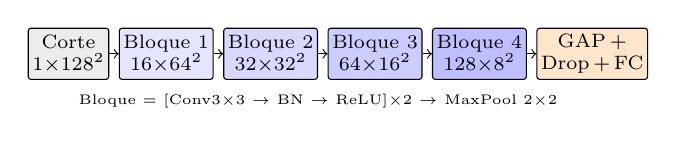
\begin{tikzpicture}[font=\scriptsize, node distance=1.2mm,
  b/.style={draw, rounded corners=1pt, minimum height=6.5mm, align=center, inner sep=1.5pt}]
\node[b, fill=gray!15] (in) {Corte\\1$\times$128$^2$};
\node[b, fill=blue!10, right=of in] (b1) {Bloque 1\\16$\times$64$^2$};
\node[b, fill=blue!15, right=of b1] (b2) {Bloque 2\\32$\times$32$^2$};
\node[b, fill=blue!20, right=of b2] (b3) {Bloque 3\\64$\times$16$^2$};
\node[b, fill=blue!25, right=of b3] (b4) {Bloque 4\\128$\times$8$^2$};
\node[b, fill=orange!20, right=of b4] (h) {GAP\,+\\Drop\,+\,FC};
\foreach \a/\c in {in/b1,b1/b2,b2/b3,b3/b4,b4/h} \draw[->] (\a) -- (\c);
\node[below=0.6mm of b2.south east, anchor=north] {\tiny Bloque $=$ [Conv3$\times$3 $\rightarrow$ BN $\rightarrow$ ReLU]$\times$2 $\rightarrow$ MaxPool 2$\times$2};
\end{tikzpicture}}
\caption{Arquitectura de la CNN propuesta (294\,228 parámetros). En cada bloque se indica el tamaño del mapa de salida.}
\label{fig:arq}
\end{figure}

\begin{figure}[t]
\centering
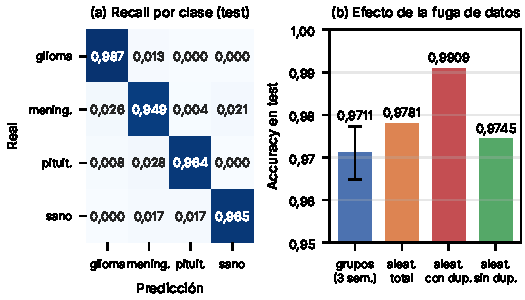
\includegraphics[width=\linewidth]{figs/cuantitativo.pdf}
\caption{(a) Matriz de confusión normalizada por fila (\textit{recall}), semilla 42. (b) \textit{Accuracy} en prueba: por grupos (media $\pm$ desv. est., 3 semillas) y aleatoria (completa y con/sin casi-duplicado en entrenamiento); el eje comienza en 0,95.}
\label{fig:cuant}
\end{figure}

\begin{figure*}[t]
\centering
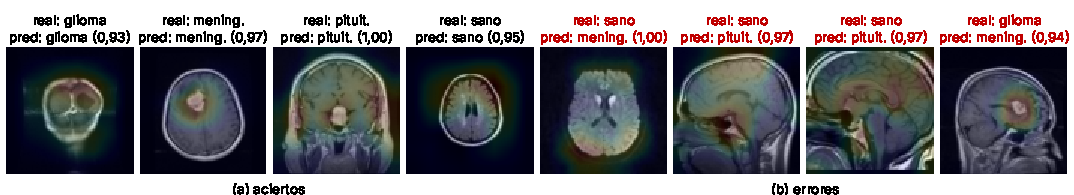
\includegraphics[width=\textwidth]{figs/cualitativo.pdf}
\caption{Ejemplos de prueba con mapa Grad-CAM superpuesto (rojo: mayor contribución a la clase predicha). (a) Un acierto por clase. (b) Los cuatro errores de mayor confianza, de grupos de casi-duplicados distintos. Se indican la clase real, la predicha y la probabilidad.}
\label{fig:cual}
\end{figure*}

\textbf{Entrenamiento.} Se usa entropía cruzada con \textit{label smoothing} 0,05~\cite{c12} y AdamW~\cite{c13} (lr $10^{-3}$, \textit{weight decay} $10^{-4}$, lote 64), con decaimiento coseno~\cite{c14} durante 30 épocas como máximo. Se guarda el modelo con mayor F1-macro de validación (paciencia 8). Se usó PyTorch con semillas fijas (CPU; 43 min la corrida principal).

\textbf{Evaluación.} Se reportan \textit{accuracy} con IC 95\,\% por \textit{bootstrap} (1\,000 remuestreos), \textit{accuracy} balanceada, F1-macro (las clases están solo levemente desbalanceadas) y AUC uno-contra-todos. En el contexto clínico se analizan el \textit{recall} por clase y los tumores clasificados como sanos. Se ejecutan dos experimentos con la misma configuración: E1 entrena con 3 semillas (42, 7, 123) para estimar media y desviación estándar; E2 entrena con la partición aleatoria y separa su prueba en imágenes con y sin casi-duplicado en entrenamiento.

\section{Resultados}
La Tabla~\ref{tab:res} resume los resultados cuantitativos. Con la partición por grupos, la CNN logra 0,9711\,$\pm$\,0,0062 de \textit{accuracy} y 0,9946\,$\pm$\,0,0008 de AUC. La semilla 42 obtiene 0,9661 (IC 95\,\%: 0,954--0,976). La brecha final entre entrenamiento y validación es de $\sim$1 punto (0,981 frente a 0,971). Por clase (Fig.~\ref{fig:cuant}a), el \textit{recall} va de 0,949 en meningioma a 0,987 en glioma. Solo 5 de 717 tumores (0,7\,\%) se clasifican como sanos, y los cinco son meningiomas. En E2, la partición aleatoria eleva el \textit{accuracy} a 0,9781. Dentro de esa prueba, las imágenes con casi-duplicado en entrenamiento alcanzan 0,9909 (2/220 errores), frente a 0,9745 (20/783) las que no lo tienen (Fig.~\ref{fig:cuant}b). Esta diferencia no es significativa con la prueba exacta de Fisher ($p=0{,}19$). Con la partición por grupos, las 55 imágenes con dHash idéntico en entrenamiento se aciertan al 100\,\% en las tres semillas, frente a 0,9694 en el resto.

\begin{table}[t]
\centering
\caption{Resultados en prueba (1\,003 imágenes) de la CNN propuesta.}
\label{tab:res}
\setlength{\tabcolsep}{2.6pt}
\begin{tabular}{|l|c|c|c|c|} \hline
\textbf{Partición / semilla} & \textbf{Acc.} & \textbf{Acc. bal.} & \textbf{F1-macro} & \textbf{AUC} \\\hline
Grupos, semilla 42  & 0,9661 & 0,9663 & 0,9657 & 0,9945 \\\hline
Grupos, semilla 7   & 0,9691 & 0,9689 & 0,9685 & 0,9938 \\\hline
Grupos, semilla 123 & 0,9781 & 0,9779 & 0,9778 & 0,9954 \\\hline
\textbf{Grupos, media} & \textbf{0,9711} & \textbf{0,9710} & \textbf{0,9707} & \textbf{0,9946} \\
\textbf{$\pm$ desv. est.} & $\pm$0,0062 & $\pm$0,0061 & $\pm$0,0063 & $\pm$0,0008 \\\hline
Aleatoria (fuga), sem. 42$^{*}$ & 0,9781 & 0,9773 & 0,9772 & 0,9989 \\\hline
\end{tabular}

\vspace{1mm}
{\scriptsize $^{*}$Evaluada en su propia partición de prueba, no comparable 1:1 con las filas anteriores.}
\end{table}





La Fig.~\ref{fig:cual} muestra los resultados cualitativos. En los aciertos de glioma, meningioma y \textit{pituitary}, la activación se concentra sobre la lesión o la región selar. Los errores de mayor confianza son sobre todo cortes sanos atípicos: una imagen axial de difusión (DWI) predicha como meningioma con probabilidad $\approx$1,00 (5 copias en prueba) y cortes sagitales T1 predichos como \textit{pituitary}. En ellos, el mapa no señala una lesión, sino estructuras de la línea media.

\section{Discusión}
La CNN compacta generaliza bien: la pequeña brecha entre entrenamiento y validación indica un buen balance sesgo-varianza~\cite{c15}. Contribuyen la regularización explícita (\textit{weight decay}, \textit{dropout}, \textit{label smoothing}~\cite{c12}) y el uso de \textit{global average pooling} en lugar de capas densas~\cite{c11}. La validación oscila con fuerza en las primeras $\sim$12 épocas y se estabiliza cuando el decaimiento coseno~\cite{c14} reduce la tasa de aprendizaje. La desviación entre semillas (0,6 puntos) es comparable al IC de una sola corrida: diferencias menores a $\sim$1 punto entre configuraciones no son concluyentes sin repetición. El resultado está en el rango de~\cite{c6} (96,56\,\%), aunque allí se usan 3 clases y validación a nivel de registro.

La clase más difícil es meningioma (\textit{recall} 0,949, precisión 0,937). Se confunde con glioma cuando la lesión es heterogénea y con \textit{pituitary} cuando está en la línea media, porque la localización, una señal que la red usa (Fig.~\ref{fig:cual}a), deja de ser discriminativa. La fuga de datos actúa en la dirección descrita por~\cite{c7}: los casi-duplicados se clasifican casi a la perfección. Aquí su magnitud es moderada (+0,7 puntos), porque solo el 22\,\% de la prueba está contaminado y el conjunto contiene cortes seleccionados y no volúmenes completos.

La principal limitación es un posible atajo~\cite{c8}: la clase sana proviene de otra fuente (Br35H~\cite{c10}): su resolución mediana es 232$\times$243\,px frente a 512$\times$512 en los tumores, su intensidad media es mayor (60 frente a 33--49) y el 69\,\% no es cuadrada, por lo que el relleno le añade bordes negros que las demás clases casi no tienen. Los errores sobre cortes sanos atípicos (Fig.~\ref{fig:cual}b) sugieren que parte de la separación sano/tumor depende de la secuencia y no de la patología. Además, sin identificador de paciente persiste una fuga residual: el 5,5\,\% de la prueba se acierta sin error, lo que infla el \textit{accuracy} en $\sim$0,2 puntos (0,9711 frente a 0,9694). A esto se suman la resolución reducida (128\,px) y la falta de un modelo preentrenado para comparar. Como mejoras se proponen: (i) comparar con una red preentrenada ajustada por \textit{fine-tuning} (p.\,ej., ResNet-18~\cite{c4}); (ii) normalizar intensidades por imagen y evaluar estratificando por secuencia o en un conjunto externo; (iii) mayor resolución, para separar mejor meningioma y glioma; y (iv) calibrar las probabilidades y fijar un umbral que minimice los falsos negativos tumor$\rightarrow$sano.

\begin{thebibliography}{99}

\bibitem{c1} D. N. Louis \textit{et al.}, ``The 2021 WHO classification of tumors of the central nervous system: A summary,'' \textit{Neuro-Oncology}, vol. 23, no. 8, pp. 1231--1251, 2021, doi: 10.1093/neuonc/noab106.
\bibitem{c2} K. Simonyan and A. Zisserman, ``Very deep convolutional networks for large-scale image recognition,'' in \textit{Proc. Int. Conf. Learn. Represent. (ICLR)}, 2015, arXiv:1409.1556.
\bibitem{c3} S. Ioffe and C. Szegedy, ``Batch normalization: Accelerating deep network training by reducing internal covariate shift,'' in \textit{Proc. Int. Conf. Mach. Learn. (ICML)}, 2015, pp. 448--456.
\bibitem{c4} K. He, X. Zhang, S. Ren, and J. Sun, ``Deep residual learning for image recognition,'' in \textit{Proc. IEEE Conf. Comput. Vis. Pattern Recognit. (CVPR)}, 2016, pp. 770--778.
\bibitem{c5} J. Cheng \textit{et al.}, ``Enhanced performance of brain tumor classification via tumor region augmentation and partition,'' \textit{PLoS ONE}, vol. 10, no. 10, Art. no. e0140381, 2015, doi: 10.1371/journal.pone.0140381.
\bibitem{c6} M. M. Badža and M. Č. Barjaktarović, ``Classification of brain tumors from MRI images using a convolutional neural network,'' \textit{Appl. Sci.}, vol. 10, no. 6, Art. no. 1999, 2020, doi: 10.3390/app10061999.
\bibitem{c7} E. Yagis \textit{et al.}, ``Effect of data leakage in brain MRI classification using 2D convolutional neural networks,'' \textit{Sci. Rep.}, vol. 11, 2021, doi: 10.1038/s41598-021-01681-w.
\bibitem{c8} R. Geirhos \textit{et al.}, ``Shortcut learning in deep neural networks,'' \textit{Nat. Mach. Intell.}, vol. 2, no. 11, pp. 665--673, 2020, doi: 10.1038/s42256-020-00257-z.
\bibitem{c9} R. R. Selvaraju, M. Cogswell, A. Das, R. Vedantam, D. Parikh, and D. Batra, ``Grad-CAM: Visual explanations from deep networks via gradient-based localization,'' in \textit{Proc. IEEE Int. Conf. Comput. Vis. (ICCV)}, 2017, pp. 618--626.
\bibitem{c10} J. Chaki, ``Brain tumor MRI dataset,'' IEEE DataPort, Jul. 2023, doi: 10.21227/1jny-g144; versión de Kaggle ``Brain Tumor (MRI Scans)'' (rm1000). [En línea]. Disponible: https://www.kaggle.com/datasets/rm1000/brain-tumor-mri-scans
\bibitem{c11} M. Lin, Q. Chen, and S. Yan, ``Network in network,'' in \textit{Proc. Int. Conf. Learn. Represent. (ICLR)}, 2014, arXiv:1312.4400.
\bibitem{c12} C. Szegedy, V. Vanhoucke, S. Ioffe, J. Shlens, and Z. Wojna, ``Rethinking the inception architecture for computer vision,'' in \textit{Proc. IEEE Conf. Comput. Vis. Pattern Recognit. (CVPR)}, 2016, pp. 2818--2826.
\bibitem{c13} I. Loshchilov and F. Hutter, ``Decoupled weight decay regularization,'' in \textit{Proc. Int. Conf. Learn. Represent. (ICLR)}, 2019, arXiv:1711.05101.
\bibitem{c14} I. Loshchilov and F. Hutter, ``SGDR: Stochastic gradient descent with warm restarts,'' in \textit{Proc. Int. Conf. Learn. Represent. (ICLR)}, 2017, arXiv:1608.03983.
\bibitem{c15} I. Goodfellow, Y. Bengio, and A. Courville, \textit{Deep Learning}. Cambridge, MA, USA: MIT Press, 2016.

\end{thebibliography}

\end{document}
